% !TeX document-id = {f19fb972-db1f-447e-9d78-531139c30778}
% !BIB program = biber

\documentclass[handout]{beamer}
%\documentclass[compress]{beamer}
\usepackage[T1]{fontenc}
\usetheme[block=fill,subsectionpage=progressbar,sectionpage=progressbar]{metropolis} 
\usepackage{graphicx}

\usepackage{wasysym}
\usepackage{etoolbox}
\usepackage[utf8]{inputenc}

\usepackage{threeparttable}
\usepackage{subcaption}

\usepackage{tikz-qtree}
\setbeamercovered{still covered={\opaqueness<1->{5}},again covered={\opaqueness<1->{100}}}


\usepackage{listings}

\lstset{
	basicstyle=\scriptsize\ttfamily,
	columns=flexible,
	breaklines=true,
	numbers=left,
	%stepsize=1,
	numberstyle=\tiny,
	backgroundcolor=\color[rgb]{0.85,0.90,1}
}



\lstnewenvironment{lstlistingoutput}{\lstset{basicstyle=\footnotesize\ttfamily,
		columns=flexible,
		breaklines=true,
		numbers=left,
		%stepsize=1,
		numberstyle=\tiny,
		backgroundcolor=\color[rgb]{.7,.7,.7}}}{}


\lstnewenvironment{lstlistingoutputtiny}{\lstset{basicstyle=\tiny\ttfamily,
		columns=flexible,
		breaklines=true,
		numbers=left,
		%stepsize=1,
		numberstyle=\tiny,
		backgroundcolor=\color[rgb]{.7,.7,.7}}}{}



\usepackage[american]{babel}
\usepackage{csquotes}
\usepackage[style=apa, backend = biber]{biblatex}
\DeclareLanguageMapping{american}{american-UoN}
\addbibresource{../../bdaca.bib}
\renewcommand*{\bibfont}{\tiny}

\usepackage{tikz}
\usetikzlibrary{shapes,arrows,matrix}
\usepackage{multicol}

\usepackage{subcaption}

\usepackage{booktabs}
\usepackage{graphicx}



\makeatletter
\setbeamertemplate{headline}{%
	\begin{beamercolorbox}[colsep=1.5pt]{upper separation line head}
	\end{beamercolorbox}
	\begin{beamercolorbox}{section in head/foot}
		\vskip2pt\insertnavigation{\paperwidth}\vskip2pt
	\end{beamercolorbox}%
	\begin{beamercolorbox}[colsep=1.5pt]{lower separation line head}
	\end{beamercolorbox}
}
\makeatother



\setbeamercolor{section in head/foot}{fg=normal text.bg, bg=structure.fg}



\newcommand{\question}[1]{
	\begin{frame}[plain]
		\begin{columns}
			\column{.3\textwidth}
			\makebox[\columnwidth]{
				
\includegraphics[width=\columnwidth,height=\paperheight,keepaspectratio]{../../pictures/mannetje.png}}
			\column{.7\textwidth}
			\large
			\textcolor{orange}{\textbf{\emph{#1}}}
		\end{columns}
\end{frame}}




\title[Big Data and Automated Content Analysis]{\textbf{Big Data \& Automated Content Analysis} \\ Week 7 -- Wednesday: »Text as data«}
\author[Anne Kroon]{Anne Kroon \\ ~ \\ \footnotesize{a.c.kroon@uva.nl \\@annekroon} \\ }
\date{10 May 2021}
\institute[UvA]{Afdeling Communicatiewetenschap \\Universiteit van Amsterdam}

\begin{document}
	
	\begin{frame}{}
		\titlepage
	\end{frame}
	
	\begin{frame}{Today}
		\tableofcontents
	\end{frame}
	
	
\begin{frame}[standout]	
	How did the exam go?
\end{frame}
	
	
	\begin{frame}[standout]	
		Everything clear from last week?
	\end{frame}
	
\section{Bag-of-words}

\subsection{General idea}

\begin{frame}[fragile]{A text as a collections of word}

Let us represent a string 
\begin{lstlisting}
t = "This this is is is a test test test"
\end{lstlisting}
like this:\\
\begin{lstlisting}
from collections import Counter
print(Counter(t.split()))
\end{lstlisting}
\begin{lstlistingoutput}
Counter({'is': 3, 'test': 3, 'This': 1, 'this': 1, 'a': 1})
\end{lstlistingoutput}

\pause 
Compared to the original string, this representation
\begin{itemize}
	\item is less repetitive
	\item preserves word frequencies
	\item but does \emph{not} preserve word order
	\item can be interpreted as a vector to calculate with (!!!)
\end{itemize}

\tiny{\emph{Of course, still a lot of stuff to fine-tune\ldots}  (for example, This/this)}
\end{frame}



\begin{frame}{From vector to matrix}
If we do this for multiple texts, we can arrange the vectors in a table.

t1 = "This this is is is a test test test" \newline
t2 = "This is an example"

\begin{tabular}{| c|c|c|c|c|c|c|c|}
	\hline
	& a & an & example & is & this & This & test \\
	\hline
	\emph{t1} & 1 & 0 & 0 & 3 & 1 & 1 & 3 \\
	\emph{t2} &0 & 1 & 1 & 1 & 0 & 1 & 0 \\
	\hline
\end{tabular}
\end{frame}


\question{What can you do with such a matrix? Why would you want to represent a collection of texts in such a way?}


\begin{frame}{The cell entries: raw counts versus tf$\cdot$idf scores}
\begin{itemize}
	\item In the example, we entered simple counts (the ``term frequency'')
\end{itemize}
\end{frame}

\question{But are all terms equally important?}


\begin{frame}{The cell entries: raw counts versus tf$\cdot$idf scores}
	\begin{itemize}
		\item In the example, we entered simple counts (the ``term frequency'')
		\item But does a word that occurs in almost all documents contain much information?
		\item And isn't the presence of a word that occurs in very few documents a pretty strong hint?
		\item<2-> \textbf{Solution: Weigh by \emph{the number of documents in which the term occurs at least once) (the ``document frequency'')}} 
	\end{itemize}
\onslide<3->{
$\Rightarrow$ we multiply the ``term frequency'' (tf) by the inverse document frequency (idf)

\tiny{(usually with some additional logarithmic transformation and normalization applied, see \url{https://scikit-learn.org/stable/modules/generated/sklearn.feature_extraction.text.TfidfTransformer.html})}
}
\end{frame}

\begin{frame}{tf$\cdot$idf}
\begin{array}{ccc}
	
	w_{i, j}=t f_{i, j} \times \log \left(\frac{N}{d f_{i}}\right)  \\ \\
	
	t f_{i, j}=\text { number of occurrences of } i \text { in } j \\
	d f_{i}=\text { number of documents containing } i \\
	N=\text {total number of documents }
\end{array}
\end{frame}

\begin{frame}{Is tf$\cdot$idf always better?}
It depends.

\begin{itemize}
	\item Ultimately, it's an empirical question which works better ($\rightarrow$ weeks on machine learning)
	\item In many scenarios,  ``discounting'' too frequent words and ``boosting'' rare words makes a lot of sense (most frequent words in a text can be highly un-informative)
	\item Beauty of raw tf counts, though: interpretability + describes document in itself, not in relation to other documents
\end{itemize}
\end{frame}


%\begin{frame}{Internal representations}
%\begin{block}{Sparse vs dense matrices}
%\begin{itemize}
%	\item $\rightarrow$ tens of thousands of columns (terms), and one row per document
%	\item Filling all cells is inefficient \emph{and} can make the matrix too large to fit in memory (!!!)
%	\item Solution: store only non-zero values with their coordinates! (sparse matrix)
%	\item dense matrix (or dataframes) not advisable, only for toy examples
%\end{itemize}
%\end{block}
%\end{frame}


%{\setbeamercolor{background canvas}{bg=black}
%	\begin{frame}
%	\makebox[\linewidth]{
%		\includegraphics[width=\paperwidth,height=\paperheight,keepaspectratio]{../../pictures/sparse_dense.png}}
%\end{frame}
%}



\section{clean BOW}

\begin{frame}{Room for improvement}
\begin{description}
	\item[tokenization] How do we (best) split a sentence into tokens (terms, words)?
	\item[pruning] How can we remove unneccessary words?
	\item[lemmatization] How can we make sure that slight variations of the same word are not counted differently?

\end{description}
\end{frame}

\subsection{Better tokenization}

\begin{frame}[fragile]{OK, good enough, perfect?}
\begin{block}{.split()}
\begin{itemize}
	\item space $\rightarrow$ new word
	\item no further processing whatsoever
	\item thus, only works well if we do a preprocessing outselves (e.g., remove punctuation)
\end{itemize}
\end{block}
\begin{lstlisting}
docs = ["This is a text",  "I haven't seen John's derring-do. Second sentence!"]
tokens = [d.split() for d in docs]
\end{lstlisting}
\begin{lstlistingoutputtiny}
[['This', 'is', 'a', 'text'], ['I', "haven't", 'seen', "John's", 'derring-do.', 'Second', 'sentence!']]
\end{lstlistingoutputtiny}
\end{frame}


\begin{frame}[fragile]{OK, good enough, perfect?}
	\begin{block}{Tokenizers from the NLTK pacakge}
		\begin{itemize}
			\item multiple improved tokenizers that can be used instead of .split()
			\item e.g., Treebank tokenizer:
			\begin{itemize}
				\item split standard contractions ("don't")
				\item deals with punctuation
			\end{itemize}			
		\end{itemize}
	\end{block}
\begin{lstlisting}
from nltk.tokenize import TreebankWordTokenizer
tokens = [TreebankWordTokenizer().tokenize(d) for d in docs]
\end{lstlisting}
\begin{lstlistingoutputtiny}
[['This', 'is', 'a', 'text'],  ['I', 'have', "n't", 'seen', 'John', "'s", 'derring-do.', 'Second', 'sentence', '!']]
\end{lstlistingoutputtiny}
\tiny{Notice the failure to split the \texttt{.} at the end of the first sentence in the second doc. That's because TreebankWordTokenizer expects \emph{sentences} as input. See book for a solution.\\}
\end{frame}


\begin{frame}[standout]
OK, so we can tokenize with a list comprehension (and that's often a good idea!). But what if we want to \emph{directly} get a DTM instead of lists of tokens?
\end{frame}


\begin{frame}[fragile]{OK, good enough, perfect?}
	\begin{block}{scikit-learn's CountVectorizer (default settings)}
		\begin{itemize}
			\item applies lowercasing
			\item deals with punctuation etc. itself
			\item minimum word length $>1$
			\item more technically, tokenizes using this regular expression: \texttt{r"(?u)\textbackslash b\textbackslash w\textbackslash w+\textbackslash b"} \footnote{?u = support unicode, \textbackslash b = word boundary}
		\end{itemize}
	\end{block}
\begin{lstlisting}
from sklearn.feature_extraction.text import CountVectorizer
cv = CountVectorizer()
dtm_sparse = cv.fit_transform(docs)
\end{lstlisting}
\end{frame}


\begin{frame}{OK, good enough, perfect?}
	\begin{block}{CountVectorizer supports more}
		\begin{itemize}
			\item stopword removal
			\item custom regular expression
			\item or even using an external tokenizer
			\item ngrams instead of unigrams
		\end{itemize}
	\end{block}
			\tiny{see \url{https://scikit-learn.org/stable/modules/generated/sklearn.feature\_extraction.text.CountVectorizer.html}}

\pause
\begin{alertblock}{Best of both worlds}
\textbf{Use the Count vectorizer with a NLTK-based external tokenizer! (see book)}
\end{alertblock}
\end{frame}



\subsection{Stopword removal}



\begin{frame}{Stopword removal}
	\begin{block}{What are stopwords?}
		\begin{itemize}
			\item Very frequent words with little inherent meaning
			\item \texttt{the, a, he, she, \ldots}
			\item context-dependent: if you are interested in gender, \texttt{he} and \texttt{she} are no stopwords. 
			\item Many existing lists as basis
		\end{itemize}
	\end{block}

When using the CountVectorizer, we can simply provide a stopword list. 

But we can also remove stopwords ``by hand'' (next slide):
\end{frame}

\begin{frame}[fragile]{Stopword removal}
\begin{lstlisting}
from nltk.corpus import stopwords
mystopwords = stopwords.words("english")
mystopwords.extend(["test", "this"])

def tokenize_clean(s, stoplist):
    cleantokens = []
    for w in TreebankWordTokenizer().tokenize(s):
        if w.lower() not in stoplist:
            cleantokens.append(w)
    return cleantokens

tokens = [tokenize_clean(d, mystopwords) for d in docs]
\end{lstlisting}
\begin{lstlistingoutputtiny}
[['text'], ["n't", 'seen', 'John', 'derring-do.', 'Second', 'sentence', '!']]
\end{lstlistingoutputtiny}

\begin{alertblock}{You can do more!}
For instance, in line 8, you could add an \texttt{or} statement to also exclude punctuation.
\end{alertblock}

\end{frame}


%
%
%
%\subsection{Pruning}
%
%\begin{frame}{General idea}
%\begin{itemize}
%	\item Idea behind both stopword removal and tf$\cdot$idf: too frequent words are uninformative
%	\item<2-> (possible) downside stopword removal: a priori list, does not take empirical frequencies in dataset into account
%	\item<3-> (possible) downside tf$\cdot$idf: does not reduce number of features
%\end{itemize}
%
%\onslide<4->{Pruning: remove all features (tokens) that occur in less than X or more than X of the documents}
%\end{frame}

\begin{frame}[fragile, plain]
CountVectorizer, only stopword removal
\begin{lstlisting}
from sklearn.feature_extraction.text import CountVectorizer, TfidfVectorizer
myvectorizer = CountVectorizer(stop_words=mystopwords)
\end{lstlisting}

CountVectorizer, better tokenization, stopword removal (pay attention that stopword list uses same tokenization!):
\begin{lstlisting}
myvectorizer = CountVectorizer(tokenizer = TreebankWordTokenizer().tokenize, stop_words=mystopwords)
\end{lstlisting}

Additionally remove words that occur in more than 75\% or less than $n=2$ documents:
\begin{lstlisting}
myvectorizer = CountVectorizer(tokenizer = TreebankWordTokenizer().tokenize, stop_words=mystopwords, max_df=.75, min_df=2)
\end{lstlisting}

All togehter: tf$\cdot$idf, explicit stopword removal, pruning
\begin{lstlisting}
myvectorizer = TfidfVectorizer(tokenizer = TreebankWordTokenizer().tokenize, stop_words=mystopwords, max_df=.75, min_df=2)
\end{lstlisting}


\end{frame}


\question{What is ``best''? Which (combination of) techniques to use, and how to decide?}



\subsection{Stemming and lemmatization}


\begin{frame}[fragile]{Stemming and lemmatization}
\begin{itemize}
\item Stemming: reduce words to its stem by removing last part (drinking $\rightarrow$ drink)
\item Lemmatization: find word that you would need to look up in a dictionary (drinking $\rightarrow$ drink, but also went $\rightarrow$ go)
\item stemming is simpler than lemmatization
\item lemmatization often better
\end{itemize}
\pause

Example below: tokenization and lemmatization with \texttt{spacy} in one go:
\begin{lstlisting}
import spacy
nlp = spacy.load('en')   # potentially you need to install the language model first
lemmatized_tokens = [[token.lemma_  for token in nlp(doc)] for doc in docs]
\end{lstlisting}
\begin{lstlistingoutputtiny}
[['this', 'be', 'a', 'text'], ['-PRON-', 'have', 'not', 'see', 'John', "'s", 'derring', '-', 'do', '.', 'second', 'sentence', '!']]
\end{lstlistingoutputtiny}
\end{frame}




\subsection{How further?}

\begin{frame}{Main takeaway}

\begin{itemize}
	\item It matters how you transform your text into numbers (``vectorization'').
	\item Preprocessing matters, be able to make informed choices.
	\item Keep this in mind when we will discuss Machine Learning. 
\end{itemize}

\begin{itemize}
	\item Once you vectorized your texts, you can do all kinds of calculations (random example: get the cosine similarity between two texts)
\end{itemize}

\end{frame}

\begin{frame}{More NLP}
\begin{description}
	\item[$n$-grams] Consider using $n$-grams instead of unigrams
%	\item[collocations]  $n$grams that appear more frequently than expected
	\item[POS-tagging] grammatical function (``part-of-speach'') of tokens
	\item[NER] named entity recognition (persons, organizations, locations)
\end{description}
\end{frame}

\begin{frame}{More NLP}
I \textbf{really} recommend looking into spacy (\url{https://spacy.io}) for advanced natural language processing, such as part-of-speech-tagging and named entity recogntion.
\end{frame}

\section{Unsupervised machine learning}


\begin{block}<3->{Unsupervised machine learning}
	You have no labels. \onslide<4>{(\footnotesize{You did not measure \texttt{y})}}\\
	\onslide<5>{\textbf{Again, you already know some techniques to find out how \texttt{x1}, \texttt{x2},\ldots \texttt{x\_i} co-occur from other courses:} \begin{itemize}
			\item Principal Component Analysis (PCA) and Singular Value Decomposition (SVD)
			\item Cluster analysis
			\item Topic modelling (Non-negative matrix factorization and Latent Dirichlet Allocation)
			\item \ldots
		\end{itemize}
	}
\end{block}





\begin{frame}{Unsupervised techniques\ldots}

\begin{enumerate}
\item Finding similar variables (dimensionality reduction) -- unsupervised
\item Finding similar cases (clustering) -- unsupervised
\end{enumerate}
\end{frame}


\begin{frame}[plain]
\begin{table}[]
\resizebox{\textwidth}{!}{%
\begin{tabular}{lllllll}
& x1 & x2 & x3 & x4 & x5 & y \\
case1 & \ding{110}  & \ding{110}  & \ding{110}  & \ding{110}  & \ding{110} & \ding{110} \\
case2 & \ding{110}  & \ding{110}  & \ding{110}  & \ding{110}  & \ding{110} & \ding{110}\\
case3 & \ding{110}  & \ding{110}  & \ding{110}  & \ding{110}  & \ding{110} & \ding{110}\\
case4 & \ding{110}  & \ding{110}  & \ding{110}  & \ding{110}  & \ding{110} & \ding{110}\\
\end{tabular}%
}
\end{table}
\end{frame}



\begin{frame}[plain]
\begin{table}[]
\resizebox{\textwidth}{!}{%
\begin{tabular}{lllllll}
& \textcolor{orange}{x1} & x2 & \textcolor{orange}{x3}& \textcolor{blue}{x4} & \textcolor{blue}{x5} & \textcolor{gray}{(y)} \\
case1 & \textcolor{orange}{\ding{110}}  & \ding{110}  & \textcolor{orange}{\ding{110}}  & \textcolor{blue}{\ding{110}} & \textcolor{blue}{\ding{110}} & \textcolor{gray}{(\ding{110})} \\
case2 & \textcolor{orange}{\ding{110}}  & \ding{110}  & \textcolor{orange}{\ding{110}}  & \textcolor{blue}{\ding{110}} & \textcolor{blue}{\ding{110}} & \textcolor{gray}{(\ding{110})} \\
case3 & \textcolor{orange}{\ding{110}}  & \ding{110}  & \textcolor{orange}{\ding{110}}  & \textcolor{blue}{\ding{110}} & \textcolor{blue}{\ding{110}} & \textcolor{gray}{(\ding{110})} \\
case4 & \textcolor{orange}{\ding{110}}  & \ding{110}  & \textcolor{orange}{\ding{110}}  & \textcolor{blue}{\ding{110}} & \textcolor{blue}{\ding{110}} & \textcolor{gray}{(\ding{110})} \\
\end{tabular}%
}
\end{table}
Dimensionality reduction: finding similar variables (features)
\end{frame}


\begin{frame}[plain]
\begin{table}[]
\resizebox{\textwidth}{!}{%
\begin{tabular}{lllllll}
& x1 & x2 & x3 & x4 & x5 & \textcolor{gray}{(y)} \\
\textcolor{orange}{case1} & \textcolor{orange}{\ding{110}}  & \textcolor{orange}{\ding{110}}  &\textcolor{orange}{\ding{110}}  &\textcolor{orange}{\ding{110}}   & \textcolor{orange}{\ding{110}} & \textcolor{gray}{(\ding{110})} \\
\textcolor{blue}{case2} & \textcolor{blue}{\ding{110}}  & \textcolor{blue}{\ding{110}}  &\textcolor{blue}{\ding{110}}  &\textcolor{blue}{\ding{110}}   & \textcolor{blue}{\ding{110}} & \textcolor{gray}{(\ding{110})} \\
\textcolor{orange}{case3} & \textcolor{orange}{\ding{110}}  & \textcolor{orange}{\ding{110}}  &\textcolor{orange}{\ding{110}}  &\textcolor{orange}{\ding{110}}   & \textcolor{orange}{\ding{110}} & \textcolor{gray}{(\ding{110})} \\
\textcolor{orange}{case4} & \textcolor{orange}{\ding{110}}  & \textcolor{orange}{\ding{110}}  &\textcolor{orange}{\ding{110}}  &\textcolor{orange}{\ding{110}}   & \textcolor{orange}{\ding{110}} & \textcolor{gray}{(\ding{110})} \\
\end{tabular}%
}
\end{table}
Clustering: finding similar cases
\end{frame}


\section{Finding similar variables}


\subsection{Principal Component Analysis}


\begin{frame}[fragile]{PCA}
Document-term matrix
\begin{lstlisting}
w1,w2,w3,w4,w5,w6 ...
text1, 2, 0, 0, 1, 2, 3 ...
text2, 0, 0, 1, 2, 3, 4 ...
text3, 9, 0, 1, 1, 0, 0 ...
...
\end{lstlisting}
{\small{These can be simple counts, but also more advanced metrics, like tf-idf scores (where you weigh the frequency by the number of documents in which it occurs)}}
	%, cosine distances, etc.}}
\pause
\begin{itemize}
	\item given a term-document matrix, easy to do with any tool
%	\item probably extremely skewed distributions
\end{itemize}

\end{frame}


\begin{frame}{PCA}
\begin{itemize}
\item related to and often confused with Factor Analysis (same menu item in SPSS -- many people who believe they run FA actually run PCA!)
\item Components are ordered (first explains most variance)
\item Components do \emph{not} necessarily carry a meaningful interpretation
\end{itemize}
\end{frame}


\begin{frame}[fragile,plain]{Running PCA}

Example of a PCA on a BOW representation of some texts:

\begin{lstlisting}
myvec = CountVectorizer(texts, max_df=.5, min_df=5)
mypca = PCA(n_components=2)

mypipe = make_pipeline(myvec, FunctionTransformer(lambda x: x.todense(), accept_sparse=True), mypca)

r = mypipe.fit_transform(texts)
\end{lstlisting}


\small{PCA does not accept a \textit{sparse matrix} as input (but the CountVectorizer gives one as output), so we need to transform it into a \textit{dense matrix}.}

\end{frame}



%\begin{frame}[fragile,plain]{Plotting the result}
%\begin{lstlisting}
%plt.scatter([e[0] for e in r], [e[1] for e in r], alpha=.6)
%\end{lstlisting}
%
%\makebox[\linewidth]{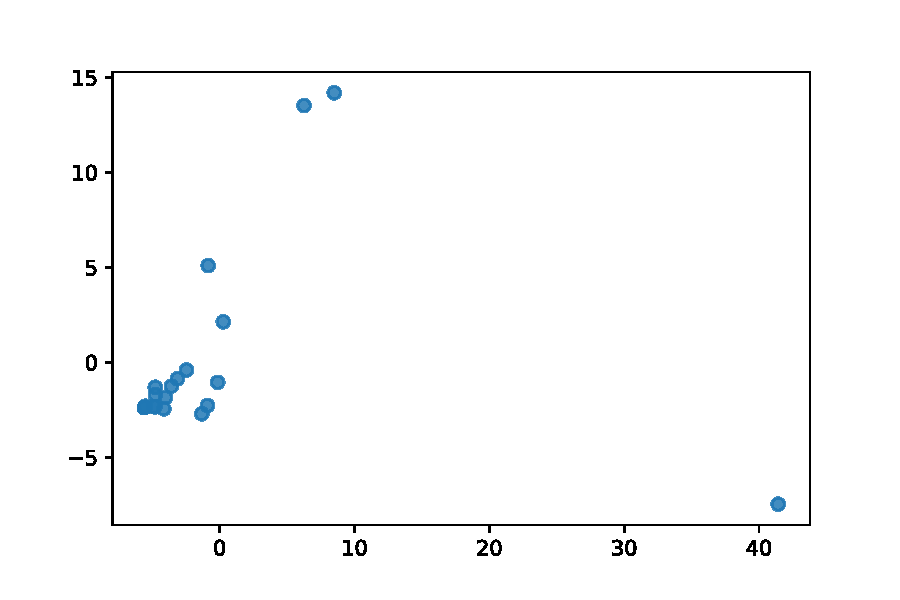
\includegraphics[width=\paperwidth,height=.6\paperheight,keepaspectratio]{../../pictures/pca-example}}
%
%
%\end{frame}
%
%
%
%\begin{frame}[fragile]{Singular value decomposition}
%The need to use a dense matrix is \emph{really} a problem for large feature sets (which we have in NLP).
%\pause
%
%We therefore can better use SVD, which is essentially* the same and very simple to use:
%
%\begin{lstlisting}
%mysvd = TruncatedSVD(n_components=2)
%mypipe = make_pipeline(myvec, mysvd)
%r = mypipe.fit_transform(texts)
%\end{lstlisting}
%
%\footnotesize{(In this specific case, we even get exactly the same plot\ldots)}
%
%
%\footnotesize{
%* It's mathematically different, but you can SVD is even used ``under the hood'' by several PCA modules to solve PCA problems.
%
%More info and background: \url{https://towardsdatascience.com/pca-and-svd-explained-with-numpy-5d13b0d2a4d8}}
%
%\end{frame}
%
%
%\begin{frame}{PCA}
%\begin{itemize}
%\item given a term-document matrix, we can easily find clusters of documents that resemble each other
%\item some problematic assumptions: \textcolor{red}{does the goal of PCA, to find a solution in which one word loads on \emph{one} component match real life, where a word can belong to several topics or frames?}
%
%\end{itemize}
%\end{frame}
%

\begin{frame}{We need other models to}
\begin{enumerate}[<+->]
\item model \emph{simultaneously} (a) which topics we find in the whole corpus, and (b) which of these topics are present in which document; while at the same time
\item allowing (a) words to be part of multiple topics, and (b) multiple topics to be present in one document
%\item being able to make connections between words ``even if they never actually occured in a document together'' (Maier et al, 2018, p.~96)
\end{enumerate}

\tiny{Maier, D., Waldherr, A., Miltner, P., Wiedemann, G., Niekler, A., Keinert, A., \ldots Adam, S. (2018). Applying LDA Topic Modeling in Communication Research: Toward a Valid and Reliable Methodology. \textit{Communication Methods and Measures, 12}(2--3), 93--118. doi:10.1080/19312458.2018.1430754}
\end{frame}



\section{LDA Topic models}

\subsection{An introduction to LDA}

\begin{frame}{}
Enter \textbf{topic modeling with Latent Dirichlet Allocation (LDA)}
\end{frame}






\begin{frame}{LDA, what's that?}
\begin{block}{No mathematical details here, but the general idea}
\begin{itemize}
\item There are $k$ topics, $T_1$\ldots$T_k$
\item Each document $D_i$ consists of a mixture of these topics, e.g.$80\% T_1, 15\% T_2, 0\% T_3, \ldots 5\% T_k $
\item On the next level, each topic consists of a specific probability distribution of words
\item Thus, based on the frequencies of words in $D_i$, one can infer its distribution of topics
\item Note that LDA (like PCA) is a Bag-of-Words (BOW) approach
\end{itemize}
\end{block}

\end{frame}




\begin{frame}[fragile]{Doing a LDA in Python}
You can use gensim ({\v R}eh{\r u}{\v r}ek \& Sojka, 2010) for this.

Let us assume you have a list of lists of words (!) called \texttt{texts}:

\begin{lstlisting}
articles=['The tax deficit is higher than expected. This said xxx ...', 'Germany won the World Cup. After a']
texts=[[token for token in re.split(r"\W", art) if len(token)>0] for art in articles]


\end{lstlisting}
which looks like this:
\begin{lstlisting}
[['The', 'tax', 'deficit', 'is', 'higher', 'than', 'expected', 'This', 'said', 'xxx'], ['Germany', 'won', 'the', 'World', 'Cup', 'After', 'a']]
\end{lstlisting}

\tiny{{\v R}eh{\r u}{\v r}ek, R., \& Sojka, P. (2010). Software framework for topic modelling with large corpora. \emph{Proceedings of the LREC 2010 Workshop on New Challenges for NLP Frameworks}, pp. 45–50. Valletta, Malta: ELRA. }

\end{frame}




\begin{frame}[plain,fragile]
\begin{lstlisting}
from gensim import corpora, models

NTOPICS = 100
LDAOUTPUTFILE="topicscores.tsv"

# Create a BOW represenation of the texts
id2word = corpora.Dictionary(texts)
mm =[id2word.doc2bow(text) for text in texts]

# Train the LDA models.
mylda = models.ldamodel.LdaModel(corpus=mm, id2word=id2word, num_topics=NTOPICS, alpha="auto")

# Print the topics.
for top in mylda.print_topics(num_topics=NTOPICS, num_words=5):
print ("\n",top)

print ("\nFor further analysis, a dataset with the topic score for each document is saved to",LDAOUTPUTFILE)

scoresperdoc=mylda.inference(mm)

with open(LDAOUTPUTFILE,"w",encoding="utf-8") as fo:
for row in scoresperdoc[0]:
fo.write("\t".join(["{:0.3f}".format(score) for score in row]))
fo.write("\n")
\end{lstlisting}

\end{frame}


\begin{frame}[fragile]{Output: Topics (below) \& topic scores (next slide)}
\begin{lstlisting}
0.069*fusie + 0.058*brussel + 0.045*europesecommissie + 0.036*europese + 0.023*overname
0.109*bank + 0.066*britse + 0.041*regering + 0.035*financien + 0.033*minister
0.114*nederlandse + 0.106*nederland + 0.070*bedrijven + 0.042*rusland + 0.038*russische
0.093*nederlandsespoorwegen + 0.074*den + 0.036*jaar + 0.029*onderzoek + 0.027*raad
0.099*banen + 0.045*jaar + 0.045*productie + 0.036*ton + 0.029*aantal
0.041*grote + 0.038*bedrijven + 0.027*ondernemers + 0.023*goed + 0.015*jaar
0.108*werknemers + 0.037*jongeren + 0.035*werkgevers + 0.029*jaar + 0.025*werk
0.171*bank + 0.122* + 0.041*klanten + 0.035*verzekeraar + 0.028*euro
0.162*banken + 0.055*bank + 0.039*centrale + 0.027*leningen + 0.024*financiele
0.052*post + 0.042*media + 0.038*nieuwe + 0.034*netwerk + 0.025*personeel
...
\end{lstlisting}
\end{frame}


\begin{frame}[plain]
\makebox[\linewidth]{
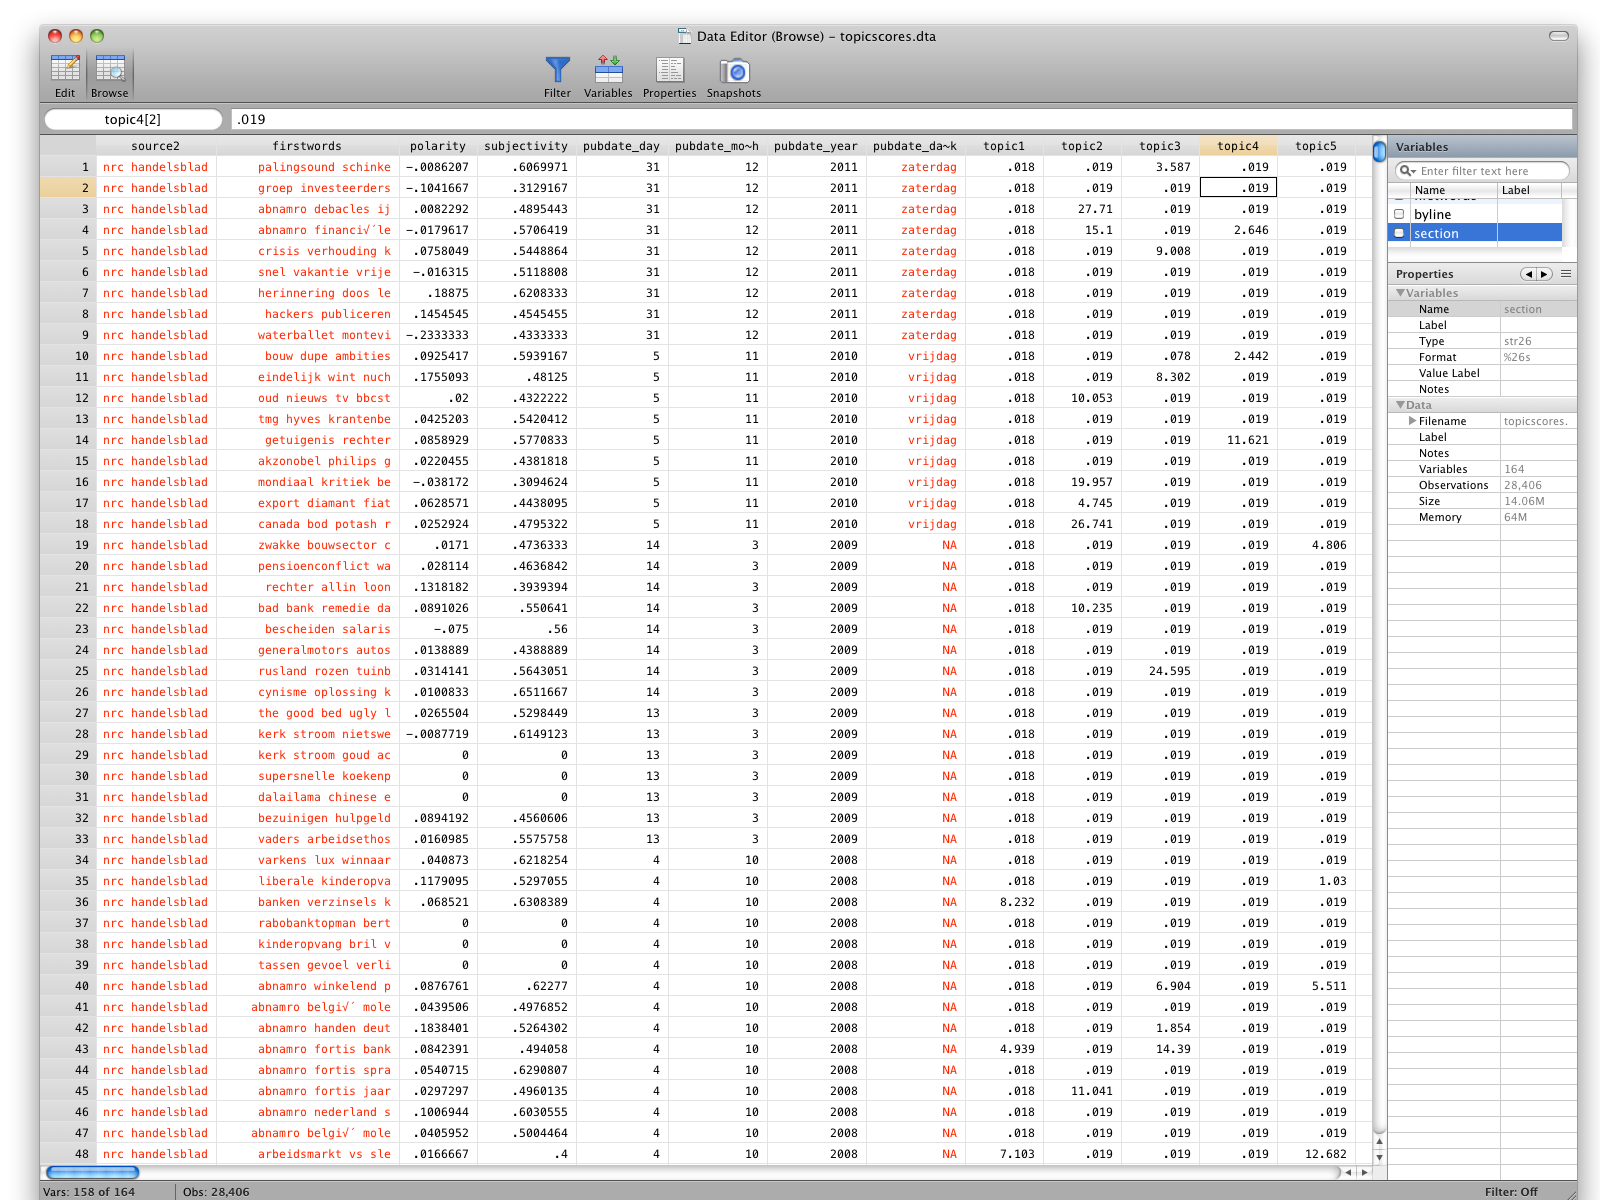
\includegraphics[width=\paperwidth,height=\paperheight,keepaspectratio]{../../pictures/topicscores}}
\end{frame}



\begin{frame}[fragile]{Visualization with pyldavis}
\begin{lstlisting}
import pyLDAvis
import pyLDAvis.gensim_models as gensimvis
# first estiate gensim model, then:
vis_data = gensimvis.prepare(mylda,mm,id2word)
pyLDAvis.display(vis_data)
\end{lstlisting}
\makebox[\linewidth]{
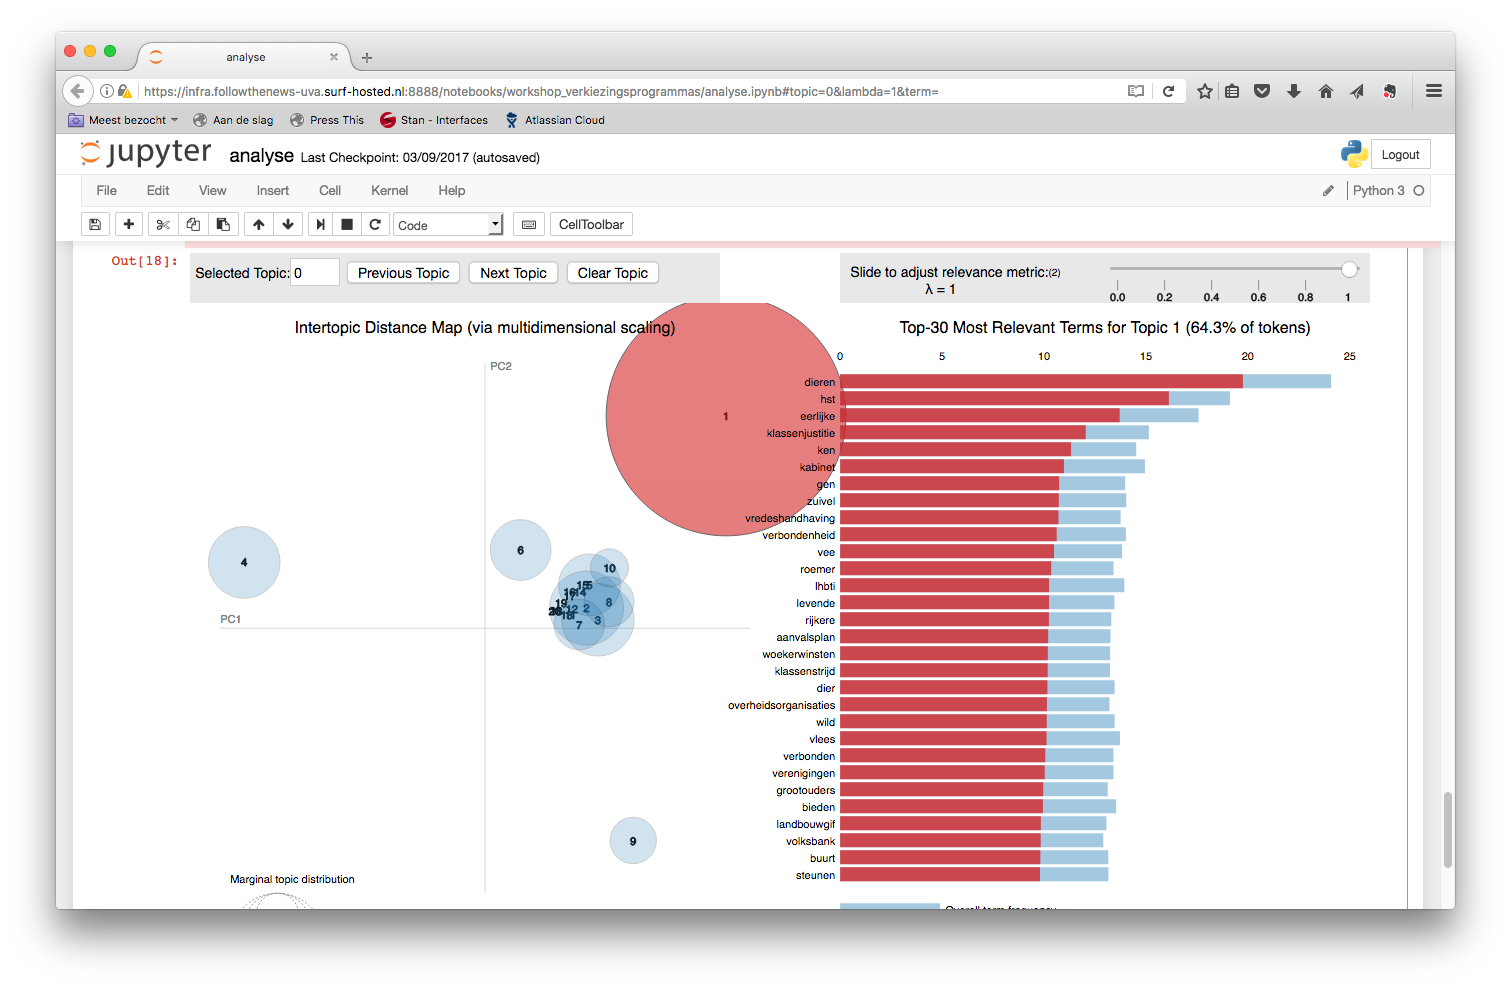
\includegraphics[width=\paperwidth,height=.5\paperheight,keepaspectratio]{../../pictures/pyldavis}}
\end{frame}

\begin{frame}{Visualization with pyldavis}
Short note about the $\lambda$ setting:

It influences the ordering of the words in pyldavis.

\begin{quote}
``For $\lambda = 1$, the ordering of the top words is equal to the ordering of the standard conditional word probabilities. For $\lambda$ close to zero, the most specific words of the topic will lead the list of top words. In their case study, Sievert and Shirley (2014, p. 67) found the best interpretability of topics using a  $\lambda$-value close to .6, which we adopted for our own case'' (Maier et al., 2018, p.~107)
\end{quote}


\tiny{Maier, D., Waldherr, A., Miltner, P., Wiedemann, G., Niekler, A., Keinert, A., \ldots Adam, S. (2018). Applying LDA Topic Modeling in Communication Research: Toward a Valid and Reliable Methodology. \textit{Communication Methods and Measures, 12}(2--3), 93--118. doi:10.1080/19312458.2018.1430754}
\end{frame}

\begin{frame}[plain]{Code examples}


\url{https://github.com/annekroon/bdaca-6ec/blob/master/6ec/week07/exercises/lda.ipynb}
\end{frame}



\subsection{Choosing the best (or a good) topic model}

\begin{frame}{Choosing the best (or a good) topic model}
\begin{itemize}
\item There is no single best solution (e.g., do you want more coarse of fine-grained topics?)
\item Non-deterministic
\item Very sensitive to preprocessing choices
\item Interplay of both metrics and (qualitative) interpretability 
\end{itemize}

See for more elaborate guidance:

\tiny{Maier, D., Waldherr, A., Miltner, P., Wiedemann, G., Niekler, A., Keinert, A., \ldots Adam, S. (2018). Applying LDA Topic Modeling in Communication Research: Toward a Valid and Reliable Methodology. \textit{Communication Methods and Measures, 12}(2--3), 93--118. doi:10.1080/19312458.2018.1430754}

\end{frame}



\begin{frame}{Evaluation metrics (closer to zero is better)}
\begin{block}{perplexity}
A goodness-of-fit measure, answering the question: If we do a train-test split, how well does the trained model fit the test data?
\end{block}

\pause 
\begin{block}{coherence}
\begin{itemize}
\item mean coherence of the whole model: attempts to quantify the interpretability
\item coherence per topic: allows to get topics that are most likely to be coherently interpreted (\texttt{.top\_topics()})
\end{itemize}
\end{block}

\end{frame}


\begin{frame}{Choosing $k$: How many topics do we want?}
\begin{itemize}
\item Typical values: $10<k<200$
\item Too low: losing nuance, so broad it becomes meaningless
\item Too high: picks up tiny pecularities instead of finding general patterns
\item There is no inherent ordering of topics (unlike PCA!)
\item We can throw away or merge topics later, so if out of $k=50$ topics 5 are not interpretable and a couple of others overlap, it still may be a good model
\end{itemize}
\end{frame}


\begin{frame}[fragile]{Choosing $\alpha$: how sparse should the document-topic distribution $\theta$ be?}
\begin{itemize}
\item The higher $\alpha$, the more topics per document 
\item Default: $1/k$
\item But: We can explicitly change it, or -- really cool -- even learn $\alpha$ from the data (\texttt{alpha = "auto"})
\end{itemize}

\pause 

Takeaway: It takes longer, but you probably want to learn alpha from the data, using multiple passes:

\begin{lstlisting}
mylda LdaModel(corpus=tfidfcorpus[ldacorpus], id2word=id2word, num_topics=50, alpha='auto', passes=10)
\end{lstlisting}


\end{frame}
%
%
%\begin{frame}{Choosing $\eta$: how sparse should the topic-word distribution $\lambda$ be?}
%\begin{itemize}
%\item Can be used to boost specific words
%\item Can also be learned from the data 
%\end{itemize}
%
%\pause
%Takeaway: Even though you can do \texttt{eta="auto"}, this usually does not help you much.
%
%\end{frame}


% \subsection{Drawbacks of LDA topic models}


\subsection{Using topic models}

\begin{frame}{Using topic models}

You got your model -- what now?

\begin{enumerate}
\item Assign topic scores to documents
\item Label topics
\item Merge/ throw away topics
\item Compare topics between, e.g., outlets
\item or do some time-series analysis.
\end{enumerate}


Example:
\tiny{Tsur, O., Calacci, D., \& Lazer, D. (2015). A Frame of Mind: Using Statistical Models for Detection of Framing and Agenda Setting Campaigns. \textit{Proceedings of the 53rd Annual Meeting of the Association for Computational Linguistics and the 7th International Joint Conference on Natural Language Processing} (pp. 1629–1638).}

\end{frame}

\section{Exercise}

\begin{frame}[plain]

\begin{block}{Exercise for this week}
	\footnotesize
	\begin{itemize}
		\item Work through the example notebook on LDA: \url{https://github.com/annekroon/bdaca-6ec/blob/master/6ec/week07/exercises/lda.ipynb}
		\item But most importantly: \textbf{Use a dataset of your choice} and find a suitable topic model.
	\end{itemize}
\end{block}

%\begin{frame}[plain]
%	\printbibliography
%\end{frame}

\end{frame}



\end{document}



